%% Short reader summary of the pre-registration. Same class and conventions as the full protocol
%% PREREG_S110_FINAL.tex and the author's preprint (aastex702, default style). The full protocol governs.
\documentclass{aastex702}
\usepackage{booktabs}
\usepackage{array}
\usepackage{graphicx}

\shorttitle{Pre-registered Sector 110 Test of TIC 4206066: Summary}
\shortauthors{Rabtsevich}
\journalinfo{Summary of the pre-registration, written before the TESS Sector 110 observations}

\newcommand{\code}[1]{\texttt{#1}}
\let\origunderscore\_
\renewcommand{\_}{\origunderscore\allowbreak}
\newcommand{\runin}[1]{\par\smallskip\noindent\textbf{#1}\enspace}

\begin{document}

\title{A Pre-registered TESS Sector 110 Test of Two Transit-like Signals in TIC 4206066: Summary}

\author[gname=Pavel,sname=Rabtsevich]{Pavel Rabtsevich}
\affiliation{Independent Researcher, Tarragona, Spain}
\email{pavel.rabtsevich.research@gmail.com}

\begin{abstract}
New TESS observations in Sector 110 will test whether two transit-like signals found earlier in TIC 4206066 recur.
The transit times, the expected depths and the analysis rules are fixed before these data exist. This summary
describes the test. The exact rules are in the full protocol v1.1 (\mbox{\code{PREREG\_S110\_FINAL.pdf}}), which
takes precedence over this summary. This summary, the full protocol and the frozen materials are archived together
at \doi{10.5281/zenodo.23175179}.
\end{abstract}

\keywords{TESS, TIC 4206066, exoplanet candidates, transit photometry, pre-registration}

\section{What is tested}

Archival TESS data of TIC 4206066 show two transit-like signals, A and B; signal B is more tentative. Both were
selected after the data had been inspected, and some analysis choices were also made after seeing the data. Sector 110
therefore gives an independent test: it shows whether the signals return at the predicted times and depths, without
any new search in period or time (Figure~\ref{fig:timeline}).

\begin{table}[ht]
\centering
\caption{Frozen predictions (rounded).\label{tab:pred}}
\begin{tabular}{@{}lrr@{}}
\toprule
Prediction & Signal A & Signal B \\
\midrule
Period (days) & 3.18278 & 11.13275 \\
Expected mean depth (ppm) & $442\pm52$ & $586\pm137$ \\
Predicted Sector 110 transits & 9 & 3 \\
\bottomrule
\end{tabular}
\end{table}

The depth is the mean drop in flux inside a fixed window around each predicted transit, in parts per million. For A,
the expected depth comes from Sectors 6 and 32; for B, it rests on a single transit in Sector 6. Both signals were
found in Sector 98, so their depths there may be inflated by selection; those depths are used only to build the upper
limit of the allowed depth range (Section~\ref{sec:data}). The predicted transit times have an uncertainty of about 4 minutes ($1\sigma$). The exact
ephemerides are in Section 3 of the full protocol and in \code{ephemeris\_final.json}.

\begin{figure*}[ht]
\centering
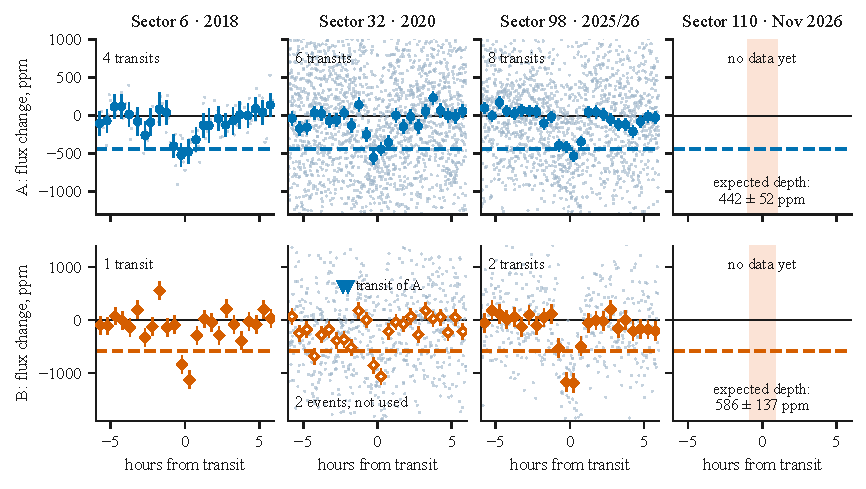
\includegraphics[width=\textwidth]{S110_transits.pdf}
\caption{Archival transits of A (top) and B (bottom), sector by sector, folded on the frozen ephemeris. Small points:
flux after the frozen detrending; large symbols: 30-minute means with their standard errors. Filled symbols use only the transits counted by the
protocol, and the dashed line is the primary expected depth. In Sector 32 no transit of B is counted: the open symbols
show its two events with data, which lie about 2 hours after transits of A and are not part of the test. The Sector
110 column stays empty until the data arrive; the shaded band is the transit window. Made by
\code{protocol\_source/make\_figure1.py} from \code{calib/expected\_depths.json}, \code{ephemeris\_final.json} and the
archival light curves.\label{fig:timeline}}
\end{figure*}

\section{Data and test} \label{sec:data}

Sector 110 is scheduled for 2026 October 31 to November 26. The test uses the first released SPOC 2-minute light
curve; the full protocol fixes the fallback light curves and when they may be used. By its own rule, this protocol counts as a
pre-registration only if it is deposited before 2026 October 31, before the Sector 110 observations begin.

Slow brightness changes are removed from the light curve, and the parts at the expected transits are left out when
these changes are estimated. The depth is then averaged over the predicted transit windows. A transit with too little
data, or one too close to a gap or to either end of the data, is ``not tested'' and does not count against the signal.

The noise is measured in the same light curve, by placing the same windows at fake transit times and processing them
in the same way. The detection threshold is the 99.9th percentile of their mean depth. The allowed depth range holds
the depths that agree with the prediction once the noise and the uncertainty of the archival depths are included.
Sensitivity is the fraction of simulated signals at the expected depth that would pass the detection threshold.

\section{Possible outcomes}

Each signal receives one primary outcome (Table~\ref{tab:out}).

\begin{table}[ht]
\caption{Outcome of each signal.\label{tab:out}}
\begin{tabular}{@{}>{\raggedright\arraybackslash}p{0.2\textwidth}>{\raggedright\arraybackslash}p{0.72\textwidth}@{}}
\toprule
Outcome & Meaning \\
\midrule
\textbf{O1 recovered} & The mean depth is above the detection threshold and inside the allowed range, and the
  timing agrees with the prediction. \\
\textbf{O2 inconsistent} & The mean depth is above the detection threshold, but the depth is outside the allowed range
  or the timing does not agree. \\
\textbf{O3 excluded} & A signal of the expected depth is excluded: the mean depth is not above the detection threshold,
  it is below the allowed range, and the sensitivity is at least 95\,\%. All three conditions are required. \\
\textbf{O4 insufficient} & The other cases defined in the full protocol, for example too few data, a non-detection
  that fails an O3 condition, or a failed primary run. The data cannot decide. \\
\bottomrule
\end{tabular}
\end{table}

A non-detection excludes a signal only when the sensitivity is at least 95\,\%, and O4 is not evidence against a
signal.

\section{Timing, position and robustness}

\runin{Timing.} The timing is checked only for a detection. One common time shift is measured for all counted
transits; it must agree with the prediction within $3\sigma$, where $\sigma$ combines the prediction and measurement
uncertainties. The check decides between O1 and O2 and cannot create a detection.

\runin{Position.} If a signal gets O1 or O2, its position on the sky is measured from the Sector 110 pixel data, with
uncertainties from artificial transits added to the same pixel data. Signal A then receives one of three labels:
compatible with the target, in tension with it, or off target. Signal B has at most three transits, so its position is
reported without a label. If the pixel data are missing or unusable, the injection checks fail, or a fallback light
curve is used, the result is ``localisation not possible''.

\runin{Robustness.} After the primary result is posted, up to six fixed processing variants are run. They never change
the primary outcome; they only decide whether an O1 or O3 may be called ``robust''. The word has a narrow meaning: at least one
variant has enough sensitivity, and none of them contradicts the primary outcome. It does not mean that all variants agree. The full
protocol lists the variants and the exact rule.

\section{Interpretation and limits}

O1 means that the predicted signal is seen again; it does not show that the signal is a planet. A position compatible
with the target cannot exclude an unresolved companion star or a background star. Low sensitivity can prevent a
decision, especially for B.

The detection threshold does not guarantee a false-alarm rate of 0.1\,\%. In archival tests on SPOC 2-minute data,
the measured false-detection rates were about 0.47\,\% for A and 0.49\,\% for B; in Sector 110 they may differ. The level for
the actual number of counted transits, given in the full protocol, is quoted with the result. These rates are not
probabilities that a signal is a planet.

\section{Materials}

The first valid primary run that writes an output file defines the primary result, and that file is posted before the
variants are run and the position is measured. A result that breaks a rule of the full protocol is invalid and cannot
be used to accept or reject a signal. All outcomes are reported, including transits that could not be tested, and any
later analysis is labelled as such. \code{PREREG\_S110\_FINAL.pdf} gives the exact rules. The ZIP file holds the
frozen code, the predictions, the calibration files and the archival checks; \code{README.md} explains how to
reproduce them, and \code{SHA256SUMS.txt} lists the checksums of all files.

\begin{acknowledgments}
AI assistance: Claude (Anthropic) assisted with drafting code and text; Codex (OpenAI) assisted with editing and
verification. The author is responsible for the protocol.
\end{acknowledgments}

\end{document}
